\documentclass[xcolor=dvipsnames,table]{beamer}

\usepackage{latexsym}
\usepackage[utf8]{inputenc}
\usepackage[brazil]{babel}
\usepackage{amssymb}
\usepackage{amsmath}
\usepackage{stmaryrd}
\usepackage{fancybox}
\usepackage{datetime}
\usepackage[T1]{fontenc}
\usepackage{graphicx}
\usepackage{graphics}
\usepackage{url}
\usepackage{algorithmic}
\usepackage{algorithm}
\usepackage{acronym}
\usepackage{array}

\newtheorem{definicao}{Definio}
\newcommand{\tab}{\hspace*{2em}}

\mode<presentation>
{
  \definecolor{colortexto}{RGB}{0,0,0}
 
  \setbeamertemplate{background canvas}[vertical shading][ bottom=white!10,top=white!10]
  \setbeamercolor{normal text}{fg=colortexto} 

  \usetheme{Warsaw}
}

\title{Definição de Linguagem \\Turing-Reconhecível} 

\author{
  Esdras Lins Bispo Jr. \\ \url{bispojr@ufg.br}
  } 
 \institute{
  Teoria da Computação \\Bacharelado em Ciência da Computação}
\date{\textbf{08 de novembro de 2017} }

\logo{
\includegraphics[width=1cm]{images/ufgJataiLogo.png}}

\begin{document}

	\begin{frame}
		\titlepage
	\end{frame}

	\AtBeginSection{
		\begin{frame}{Sumário}%[allowframebreaks]{Sumário}
    		\tableofcontents[currentsection]
    		%\tableofcontents[currentsection, hideothersubsections]
		\end{frame}
	}

	\begin{frame}{Plano de Aula}
		\tableofcontents
		%\tableofcontents[hideallsubsections]
	\end{frame}
	
	
%------------------------------------------
	\section{Revisão}
	\subsection{Configuração de MT}
	\begin{frame}{Configuração de uma MT}
		Uma configuração de uma MT leva em consideração:
		\begin{itemize}
			\item o estado atual da MT;
			\item o conteúdo atual da fita;
			\item a posição atual da cabeça.
		\end{itemize}
		\begin{block}{Uma forma especial de representar...}
			{\tt u}$q${\tt v} em que
			\begin{itemize}
				\item {\tt u} e {\tt v} são cadeias sobre $\Gamma$;
				\item {\tt uv} é o conteúdo atual da fita;
				\item $q$ é o estado atual; e
				\item a posição atual da cabeça está sobre o primeiro símbolo de {\tt v}.
			\end{itemize}
		\end{block}
	\end{frame}	
	
	\begin{frame}{Configuração de uma MT}
		\begin{center}
			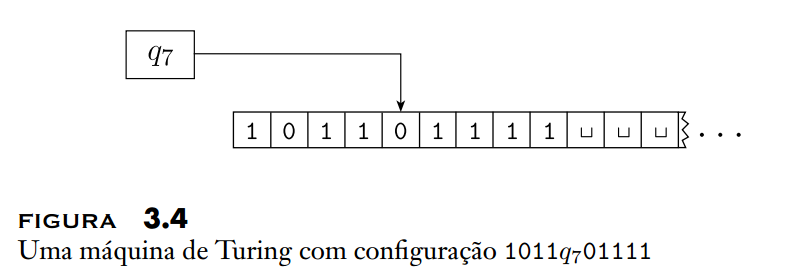
\includegraphics[height=4cm]{images/fig34.png}
		\end{center}
	\end{frame}
	
	\begin{frame}{Configuração de uma MT}
		A configuração $C_1$ {\bf origina} a configuração $C_2$, se a máquina de Turing puder legitimamente ir de $C_1$ para $C_2$.
		\begin{block}{Mais formalmente...}					Para:
			\begin{itemize}
				\item {\tt a, b, c} $\in \Gamma$,
				\item {\tt u, v} $\in \Gamma^*$, 
				\item os estados $q_i$ e $q_j$, 
				\item as configurações {\tt ua}$q_i${\tt bv} e {\tt u}$q_j${\tt acv}.
			\end{itemize}
			 	
			Digamos que 
			\begin{center}
				{\tt ua}$q_i${\tt bv} origina {\tt u}$q_j${\tt acv} 
			\end{center} 
			se na função de transição $\delta(q_i, b) = (q_j, c, E)$.
		\end{block}
	\end{frame}
	
	\begin{frame}{Configuração de uma MT}
		\begin{block}{Mais formalmente...}
			Digamos que 
			\begin{center}
				{\tt ua}$q_i${\tt bv} origina {\tt u}$q_j${\tt acv} 
			\end{center} 
			se na função de transição $\delta(q_i, b) = (q_j, c, E)$. Ou
			\begin{center}
				{\tt ua}$q_i${\tt bv} origina {\tt uac}$q_j${\tt v} 
			\end{center} 
			se na função de transição $\delta(q_i, b) = (q_j, c, D)$.
		\end{block}
	\end{frame}
	
	\begin{frame}{Configuração de uma MT}
		Termos importantes:
		\begin{itemize}
			\item configuração inicial;
			\item configuração de aceitação;
			\item configuração de rejeição;
			\item configuração de parada.
		\end{itemize}
	\end{frame}
	
	\begin{frame}{Linguagem de uma MT}
		Uma máquina de Turing $M$ {\bf aceita} a entrada $\omega$ se uma sequência de configurações $C_1, C_2, \ldots, C_k$ existe, de forma que 
		\begin{itemize}
			\item $C_1$ é a configuração inicial de $M$ sobre a entrada $\omega$;
			\item cada $C_i$ origina $C_{i+1}$;
			\item $C_k$ é uma configuração de aceitação.
		\end{itemize}  
		
		\begin{block}{Linguagem de $M$}
			É a coleção de cadeias que $M$ aceita. Também chamada de {\bf linguagem reconhecida por $M$} e denotada por $L(M)$.
		\end{block}		
	\end{frame}

	\section{Linguagem Turing-Reconhecível}	
	\begin{frame}{Definições}
		\begin{block}{Definição}
			Chame uma linguagem de {\bf Turing-reconhecível}, se alguma máquina de Turing a reconhece.
		\end{block}  \pause
		\begin{block}{Definição}
			Chame uma linguagem de {\bf Turing-decidível}, se alguma máquina de Turing a decide.
		\end{block} \pause
		\begin{block}{Corolário}
			Toda linguagem Turing-decidível é Turing-reconhecível.
		\end{block}
	\end{frame}		
	
	\begin{frame}{Exemplos}
		Uma máquina de Turing $M_2$ que decide $A = \{ 0^{2^n} \mbox{ | } n \geq 0 \}$:  
		\begin{center}
			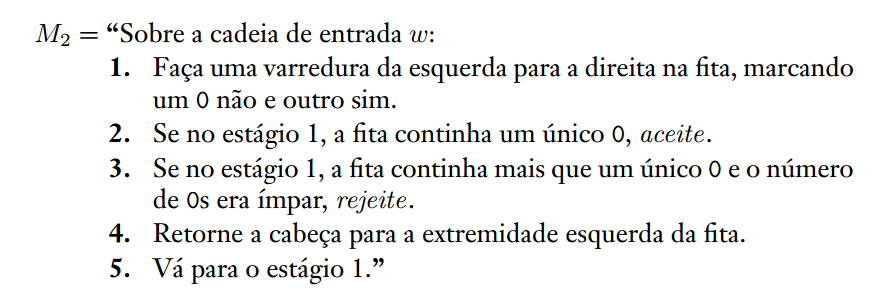
\includegraphics[height=3.5cm]{images/m2.png}
		\end{center}
	\end{frame}
	
	\begin{frame}{Exemplos}
		\begin{block}{Descrição Formal de $M_2$}
			$M_2 = (Q, \Sigma, \Gamma, \delta, q_1, q_{aceita}, q_{rejeita})$:
			\begin{itemize}
				\item $Q = \{ q_1, q_2, q_3, q_4, q_5, q_{aceita}, q_{rejeita} \}$;
				\item $\Sigma = \{ 0 \}$,
				\item $\Gamma = \{ 0, x, \sqcup \}$,
				\item Descrevemos $\delta$ no próximo slide; e
				\item $q_1, q_{aceita}$ e $q_{rejeita}$ são o estado inicial, de aceitação e de rejeição, respectivamente.
			\end{itemize}
		\end{block}
	\end{frame}
	
	\begin{frame}{Exemplos}
		\begin{center}
			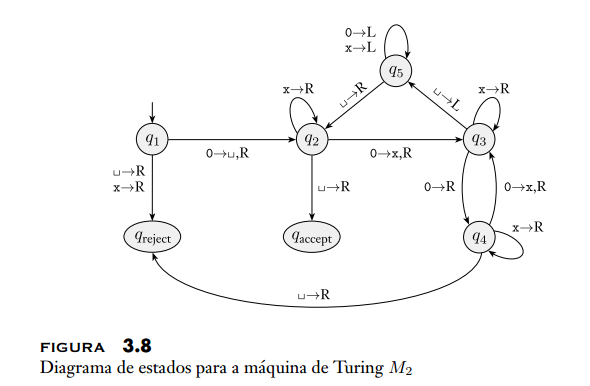
\includegraphics[height=7cm]{images/fig38.png}
		\end{center}
	\end{frame}
	
	\begin{frame}{Exemplos}
		\begin{block}{$L(M_1)$}
			Uma máquina de Turing $M_1$ que decide $B = \{ \omega \# \omega \mbox{ | } \omega \in \{ 0, 1 \}^* \}$		
		\end{block}  \pause
		\begin{block}{Descrição Formal de $M_1$}
			$M_3 = (Q, \Sigma, \Gamma, \delta, q_1 q_{aceita}, q_{rejeita})$:
			\begin{itemize}
				\item $Q = \{ q_1, \ldots, q_{14}, q_{aceita}, q_{rejeita} \}$;
				\item $\Sigma = \{ 0, 1, \# \}$,
				\item $\Gamma = \{ 0, 1, \#, x, \sqcup \}$,
				\item Descrevemos $\delta$ no próximo slide; e
				\item $q_1, q_{aceita}$ e $q_{rejeita}$ são o estado inicial, de aceitação e de rejeição, respectivamente.
			\end{itemize}
		\end{block}
	\end{frame}
	
	\begin{frame}{Exemplos}
		\begin{center}
			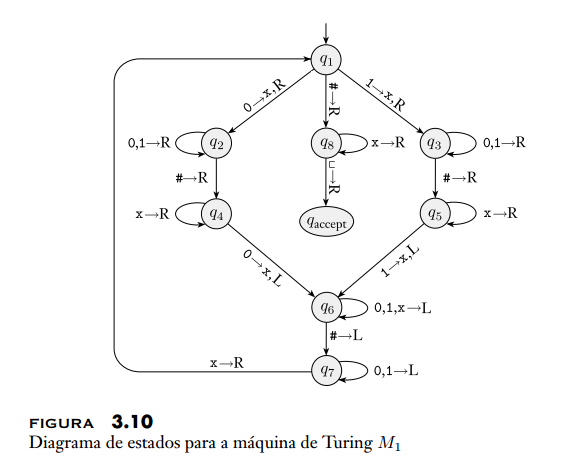
\includegraphics[height=7cm]{images/fig310.png}
		\end{center}
	\end{frame}
	
	\begin{frame}
		\titlepage
	\end{frame}
	
\end{document}